\documentclass{exam}

\usepackage{units} 
\usepackage[fleqn]{amsmath}
\usepackage{float}
\usepackage{mdwlist}
\usepackage{booktabs}
\usepackage{caption}
\usepackage{fullpage}
\usepackage{enumerate}
\usepackage{graphicx}

\usepackage{2in1, lscape} 

\everymath{\displaystyle}

\author{}
\date{January 22, 2014}
\title{Statistics \\ Week One}

\begin{document}

  \maketitle
  \tableofcontents
  \section{Homework 1}

  \begin{itemize}
    \item Histograms are always counts on the y access and thing being counted on the x
      axis.   A few people did bar chart of fish oil.

    \item draw histogram of old coins

    \item bigger bin size sometimes gives more information and takes less work
  \end{itemize}

  \section{Coin Flips}

  Flip coin 10 times and count how many heads occur.

  \begin{figure}[H]
    \centering
    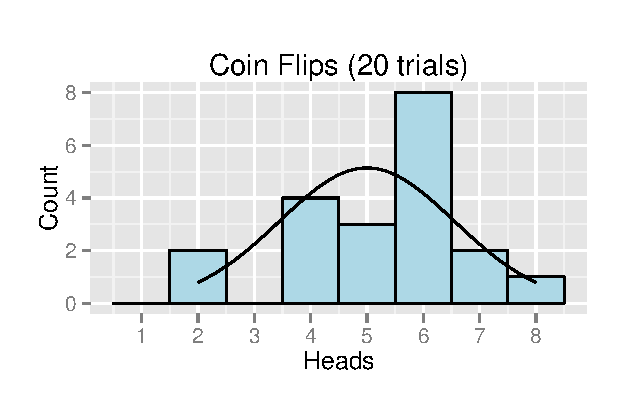
\includegraphics{figures/coins/20_10.eps}
    \caption{20 trials}
  \end{figure}

  \begin{figure}[H]
    \centering
    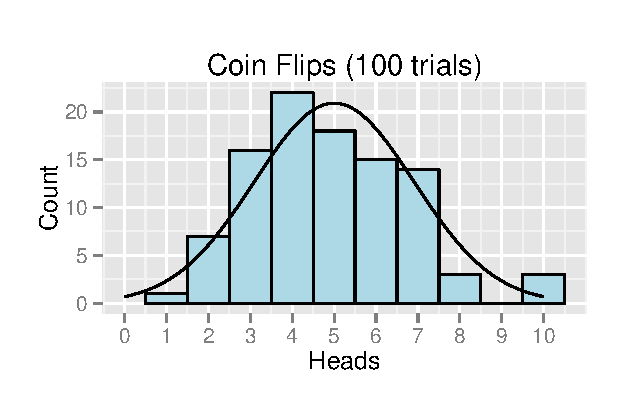
\includegraphics{figures/coins/100_10.eps}
    \caption{100 trials}
  \end{figure}

  \begin{figure}[H]
    \centering
    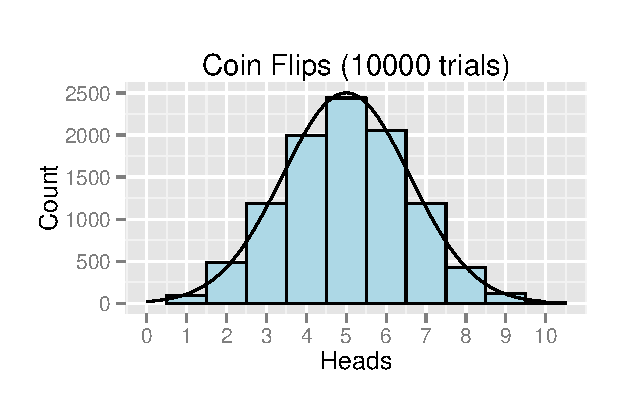
\includegraphics{figures/coins/10000_10.eps}
    \caption{10,000 trials}
  \end{figure}

  With 10,000 trials, all heads came up 8 times and all tails came up 7 times.

  \begin{table}[ht]
    \centering
    \begin{tabular}{rr}
      \toprule
      Min.    & 0.00 \\
      1st Qu. & 4.00 \\
      Median  & 5.00 \\
      Mean    & 5.01 \\
      3rd Qu. & 6.00 \\
      Max.    & 10.00 \\
      s       & 1.58441 \\
      \bottomrule
    \end{tabular}
  \end{table}

  \begin{figure}[H]
    \centering
    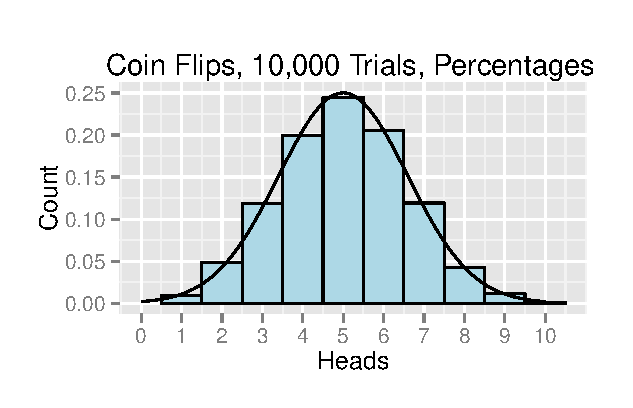
\includegraphics{figures/coins/10000_10_percent.eps}
    \caption{10,000 trials, percentages}
  \end{figure}

  \begin{figure}[H]
    \centering
    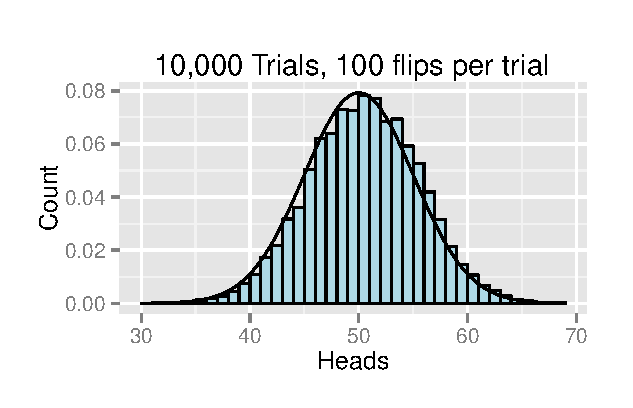
\includegraphics{figures/coins/10000_100.eps}
    \caption{10,000 trials, 100 flips per trial, percentages}
  \end{figure}

  \section{Exercise 50}
  If you do a histogram with a bin width of 100, the distribution looks like there
  is a normal distribution.

  \begin{figure}[H]
    \centering
    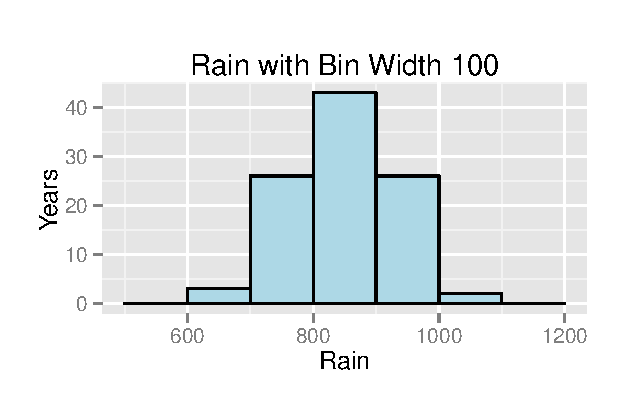
\includegraphics{figures/ex50_histogram_100.eps}
    \caption{Exercise 50 Histogram (bin width 100)}
  \end{figure}

  Here's the five number summary:
  \begin{table}[H]
    \centering
    \begin{tabular}{rr}
      \toprule
      Min.    & 651 \\
      1st Qu. & 788 \\
      Median  & 861 \\
      3rd Qu. & 905 \\
      Max.    & 1020 \\
      \bottomrule
    \end{tabular}
    \caption{Exercise 50 Summary}
  \end{table}

  The mean is smaller than the median:
  \begin{table}[H]
    \centering
    \begin{tabular}{rr}
      \toprule
      Mean    & 848 \\
      Median  & 861 \\
      \bottomrule
    \end{tabular}
    \caption{Exercise 50 mean and median}
  \end{table}

  The gaps are bigger on the low end:
  \begin{table}[H]
    \centering
    \begin{tabular}{lr}
      \toprule
      median to first quartile & 73 \\
      median to third quartile & 44 \\
      \midrule
      median to minimum & 210 \\
      median to maximum & 159 \\
      \bottomrule
    \end{tabular}
    \caption{Exercise 50 Gaps}
  \end{table}

  You can also see this in the box plot:
  \begin{figure}[H]
    \centering
    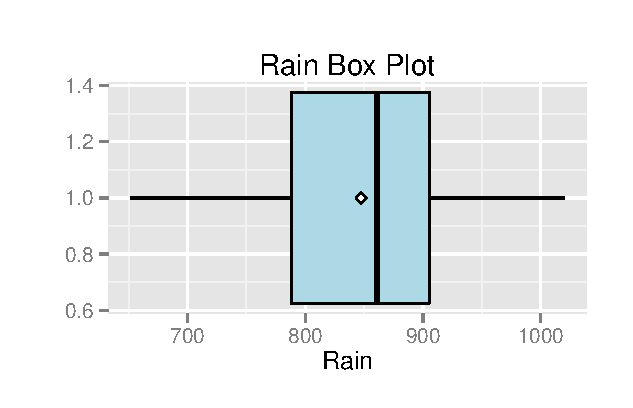
\includegraphics{figures/ex50_box.eps}
    \caption{Exercise 50 box plot}
  \end{figure}

  A histogram with smaller bin width shows that the distribution is left skewed.
  \begin{figure}[H]
    \centering
    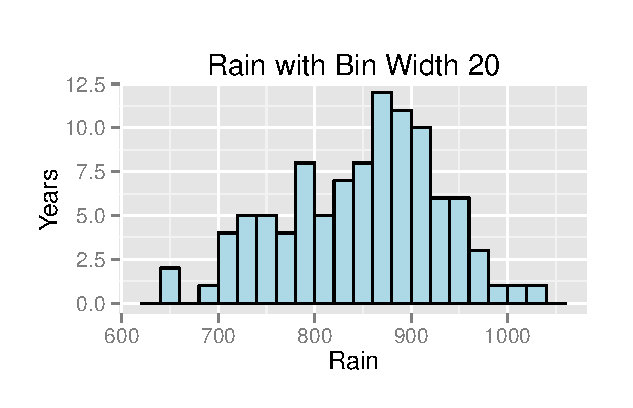
\includegraphics{figures/ex50_histogram_20.eps}
    \caption{Exercise 50 Histogram (bin width 20)}
  \end{figure}

\end{document}

